\NeedsTeXFormat{LaTeX2e}
\documentclass[12pt,a4paper,titlepage]{article} 
\usepackage[T1]{fontenc}
\usepackage{graphicx} 
\usepackage[english]{babel}
\usepackage{epsfig} 
\usepackage{subfigure} 
\usepackage{babel} 
\usepackage{epic} 
\usepackage{amsmath} 
\usepackage{float}
\usepackage[utf8]{inputenc}
%\usepackage{fancyunits}
\usepackage{hyperref}\hypersetup{colorlinks=true,linkcolor=blue,urlcolor=blue,citecolor=blue}
\usepackage{listings}
\usepackage{eurosym}
\usepackage{verbatim}
\lstset{backgroundcolor=\color[gray]{.9},
         basicstyle=\scriptsize,
         numbers=left,
	 breaklines=true
}
\selectlanguage{english} \frenchspacing \sloppy 
\usepackage{amsmath}
\usepackage{pdflscape}
\usepackage{tikz}
\usepackage{units}
\usepackage{tabularx}
\usepackage{bytefield}

% separate page numbering for title page and table of contents
\pagenumbering{roman}


% no indents
\parindent 0pt

% sans serif
\renewcommand*\familydefault{\sfdefault}

% custom date
\usepackage{datetime}
\newdateformat{customdate}{\monthname{ }\THEYEAR}

% add html links to footnoted urls
%\usepackage{html}
\renewcommand{\htmladdnormallinkfoot}[2]{#1{\footnote{\htmlurl{#2}}}}

\title{Clock Synchronisation over the Ultra Leightweight Fault Tolerant Real Time Protocol}
\newcommand{\subject}{The Ultra Leightweight Fault Tolerant Real Time Protocol}
\author{Robert Annessi, Alexander Heinisch, Nick Mayerhofer}
\date{November 2011}

% configure pdf attachments
\usepackage{attachfile}
\attachfilesetup{author=\author,icon=Paperclip,mimetype=text/plain,color=1 0 0,appearance=false}


% new line after paragraph
\makeatletter
\renewcommand\paragraph{\@startsection{paragraph}{4}{\z@}%
  {-3.25ex\@plus -1ex \@minus -.2ex}%
  {1.5ex \@plus .2ex}%
  {\normalfont\normalsize\bfseries}}
\makeatother

\newtheorem{req}{Req}


% FIXME
%\hypersetup{unicode=true,pdftitle=\title,pdfauthor=\author,pdfsubject=\subject,pdfcreator=LaTeX,pdfproducer=pdfTeX,
%pdfkeywords={}}

\begin{document} 

%\input{chapters/000_deckblatt}

\maketitle

\thispagestyle{empty}
\tableofcontents
\thispagestyle{empty}
\listoffigures
\listoftables
\newpage


\pagenumbering{arabic}

\section{Project Goal}

\subsection{Basic Idea}
The basic idea of our project is to evaluate different distributed clock synchronization algorithms over an 
asynchronous bus communication. Therefore we are going to implement a CSMA/CA protocol providing basic fault 
tolerance methods and an easy way to estimate message round trip time and message priority.
Upon the protocol, detailed described in \cite[NESD2]{NESD2}, we settle the algorithms for the clock synchronization.\\

The basic idea of our project is to evaluate different distributed clock synchronization algorithms over an 
asynchronous bus communication. Therefore we are going to implement a CSMA/CA protocol providing basic fault 
tolerance and and message priorities. Besides it should be easy to estimate the message round trip time.
Upon the protocol, described in \cite[NESD2]{NESD2} in detail, we settle the algorithms for the clock synchronization.\\

Each node has divers hardware such as buttons, LEDs, a bulb, a LCD and other peripheral components. 
We want to display drift rates of clocks on the LCD, trigger faults in the nodes internal clock and  
cause bus overloads with the connected buttons.\\

The outcome of this project should be bus protocol, which can be used by hobbyists and semi-professionals. 
We hope to gain more experience in the field of asynchronous real time bus engineering and 
to be able to estimate influences of overloads and faults to applications upon them.
We try to give a link between theoretical and practical aspects and how they relate.


\subsection{Requirements}
The requirements outlined below are an abstract view, valid for the global project idea.

\paragraph{Bus Protocol}
\begin{req}
\label{req:ulftrtp:analyzeable}
\textbf{Analyzable}: The protocol has to be easy to analyze with respect to worst case timing.
\end{req}

\begin{req}
\label{req:ulftrtp:interfacing}
\textbf{Interfacing}: The protocol design has to strictly follow interface guidelines. This means:
\begin{enumerate}
 \item Lower levels of the protocol can only be accessed by higher levels through defined layer interfaces.
 \item Higher levels of the protocol cannot be accessed by lower levels. Data can only be propagated to higher layers using callback mechanisms. 
\end{enumerate}
\end{req}

\begin{req}
\label{req:ulftrtp:easy migration}
\textbf{Migration}: The protocol has to be migratable for arbitrary applications with minimal effort.
\end{req}

\begin{req}
\label{req:ulftrtp:resource consumption}
\textbf{Resource consumption}: The protocol has to be adaptable to minimal hardware constraints.
\end{req}


\paragraph{Clock Synchronization}
\begin{req}
\label{req:clock:analyzeable}
\textbf{Analyzable}: The clock synchronization has to be easy to analyze.
\end{req}

\begin{req}
\label{req:clock:exchangeable}
\textbf{Exchangeable}: The specific clock synchronization algorithms have to be easily interchangeable with other 
clock synchronization algorithms, as we want to try out different algorithms. This Requirement correlates with 
Requirement \ref{req:ulftrtp:interfacing}.
\end{req}


\section{Project Management}

\subsection{Roles}

\textbf{Chief Executive Officer - CEO}

The duty of the CEO (or Projectmanager) is to monitor and adapt the tasks progresses and the timeplan, 
to justify deadlinemisses or delays in the development process.\\

The projectmanager also has to formulate a contract specification declaring certain requirements, 
claims, need to haves and nice to haves as well as to construct testcases in cooperation with the project 
team and the project partners.\\

Beside the depicted duties of the CEO, he/she is also responsible for project internal coordination, 
needed appointments and the assignment and monitoring of certain tasks.\\

\textbf{Chief Technical Officer - CTO}

The CTO is responsible to evaluate existing algorithms and protocols relating to the certain 
tasks as well as the design of the protocol and algorithms used in the application.\\

Another important task of the technical manager is to check the technically feasibility 
of the application or parts of it and to provide plannings and adaptions to technical contents.\\

By providing the outlined responsibilities the CTO has to be the last instance with respect to technical decisions.\\


\textbf{Chief Documentation Officer - CDO}

The CDO is responsible for the documentation process all over the project. 
His/Her aim is to provide a well structured documentation to monitor the documentation progress during coding, 
the compliance of the code with predetermined coding-guidelines.\\

Besides this he/she is responsible for codereviews, meeting protocols, and test protocols.\\

\textbf{collective responsibilities}

All project members are in charge to hand in their duties and responsibilities in time and as defined (as possible), 
to recheck decisions taken and to review, document and test their implementations on their own before handing in.\\

Reviews of documents, design decisions and implementations have to be rechecked by 
other project members as far as necessary. 
The final tests on certain implementations before assuming these valid have to be done by project members not involved in the implementation.\\

\subsection{Role allocation}

{%
\newcommand{\mc}[3]{\multicolumn{#1}{#2}{#3}}
\begin{center}
\begin{tabular}{ll}
\mc{1}{c}{\textbf{Description}} & \mc{1}{c}{\textbf{Allocation}}\\
CEO (Project Manager) & Robert Annessi\\
CTO (Technical Manager) & Alexander Heinisch\\
CDO (Documentation Manager) & Nick Mayerhofer
\end{tabular}
\end{center}
}%

\newpage


\section{Project time schedule}

We elected EGroupware for our project management matters which provides:
\begin{itemize}
 \item Time management
 \item Issue tracking
 \item Todo management and
 \item Cost tracking
\end{itemize}

\begin{landscape}
\begin{figure}[H]
 \centering
% 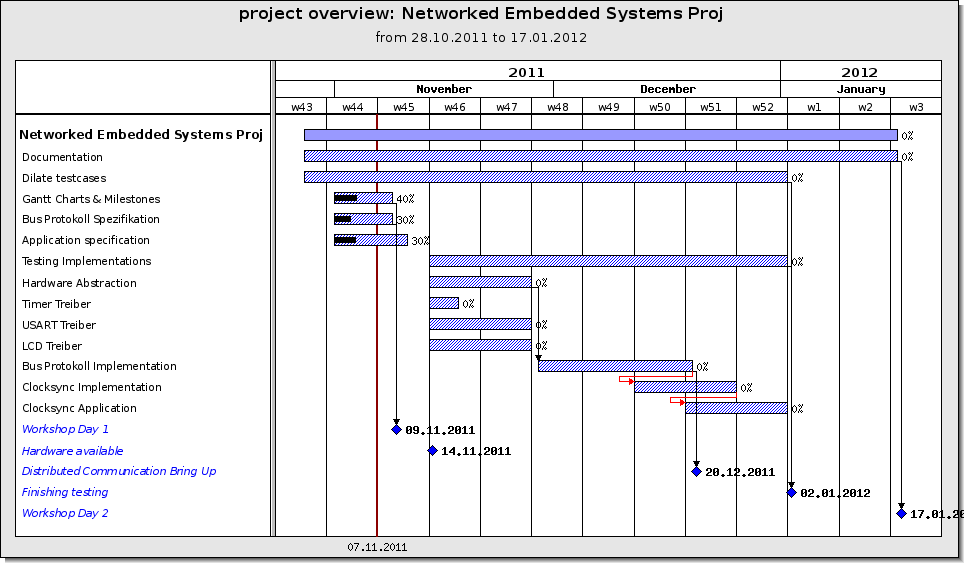
\includegraphics[angle=90,scale=0.6,keepaspectratio=true]{../images/201111_ganttchart.png}
 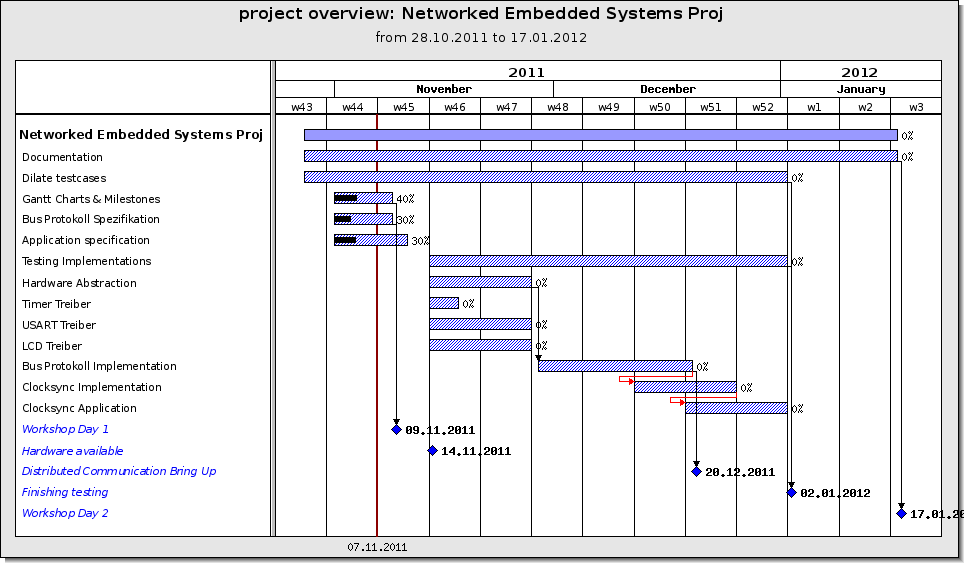
\includegraphics[scale=0.6,keepaspectratio=true]{../images/201111_ganttchart.png}
 % 201111_ganttchart.png: 964x563 pixel, 72dpi, 34.01x19.86 cm, bb=
 \caption{Gantt chart and time schedule}
 \label{fig:gantt chart}
\end{figure}
\end{landscape}

The gantt chart shown in figure \ref{fig:gantt chart} was exported from our project management tool and is described in the following sections.\\

\textbf{Legend:} \\
\begin{tabular}{lcl}
Start & ... & Planned starting date of the concerning task\\
End   & ... & Planned finishing date of the concerning task\\ 
Resources & ... & Expected resource consumption in percent\\
\end{tabular}


\subsection{Project presentation}
\begin{wrapfigure}{r}{0mm}
\begin{tabular}[t]{|lr|}
\hline
Start & kw43\\
End & kw46\\
Resources[\%] & 5\\
\hline
\end{tabular}
\end{wrapfigure}
Project presentation for the first workshop day.


\subsection{Documentation}
\begin{wrapfigure}{r}{0mm}
\begin{tabular}[t]{|lr|}
\hline
Start & kw43\\
End & kw3\\
Resources[\%] & 40\\
\hline
\end{tabular}
\end{wrapfigure}
Documentation is one of the main parts of project and refers to the entire project 
process flow and therefore lives over the entire project.\\
One of the main parts in this project is project management and we attach much 
importance to it and thus also on the documentation.\\

Documentation consists of: the documents \cite [NESD1]{NESD1} - \cite [NESD5]{NESD5} 
as well as in code documentation with doxygen.

\subsection{Dilate testcases}
\begin{wrapfigure}{r}{0mm}
\begin{tabular}[t]{|lr|}
\hline
Start & kw43\\
End & kw3\\
Resources [\%] & 10\\
\hline
\end{tabular}
\end{wrapfigure}
The matter of dialating testcases is to provide appropriate sets of conditions or variables under which
a tester is able to determine whether the application is working correctly or not.

Our test cases will include a description of the functionality to be tested and the preparation required
to ensure that the test can be conducted.\\
We will test our system in case of bus load and clock drifts so that we are able to get
significant test results to ensure our clocks can be synchronized in case of a high bus load.

\subsection{Gantt Charts \& Milestones}
\begin{wrapfigure}{r}{0mm}
\begin{tabular}[t]{|lr|}
\hline
Start & kw44\\
End & kw45\\
Resources [\%] & 5\\
\hline
\end{tabular}
\end{wrapfigure}
We are providing a Gantt Chart - that is a task dependent timeline - in form of a image output of our 
project management tool eGroupware. That includes milestones which are points 
in time bounded to the timelines in the Gantt Chart.
\subsection{Bus protocol specification}
\begin{wrapfigure}{r}{0mm}
\begin{tabular}[t]{|lr|}
\hline
Start & kw44\\
End & kw45\\
Resources [\%] & 10\\
\hline
\end{tabular}
\end{wrapfigure}
Our bus protocol specification provides a well structured communication interface and can be found in the document \cite [NESD2]{NESD2}.

It describes the operational purpose and the qualities of our bus protocol.
\subsection{Testing Implementations}
\begin{wrapfigure}{r}{0mm}
\begin{tabular}[t]{|lr|}
\hline
Start & kw46\\
End & kw52\\
Resources [\%] & 5\\
\hline
\end{tabular}
\end{wrapfigure}
Over the real process of implementation the hole team has to take care that their 
implementations are tested with the concerning testcase or with a miniature subset of a testcase.\\

Testing each implementation is an important part of the implementation an takes place during the implementation.

\subsection{Hardware Abstraction}
\begin{wrapfigure}{r}{0mm}
\begin{tabular}[t]{|lr|}
\hline
Start & kw46\\
End & kw48\\
Resources [\%] & 5\\
\hline
\end{tabular}
\end{wrapfigure}
Hardware abstraction includes the particular parts of concrete hardware APIs needed through the project. 
That means that the hardware abstraction layer (HAL) makes high level programming interfaces available to 
higher abstraction layers.

We broke down our main hardware parts to:
\begin{itemize}
 \item Timer driver\\
Which allows to initialize, set and get hardware timer concerning values that are needed
for further use regarding our bus communication, clock, clock synchronization and 
measurements concerning drift rates
 \item USART driver\\
Which allows us to arbitrate the bus and to send and receive data over the bus.
 \item LCD driver\\
Which allows us to initialize and draw text to the LC-Display.
\end{itemize}

\subsection{Bus Protocol Implementation}
\begin{wrapfigure}{r}{0mm}
\begin{tabular}[t]{|lr|}
\hline
Start & kw48\\
End & kw51\\
Resources [\%] & 10\\
\hline
\end{tabular}
\end{wrapfigure}
The bus protocol is the second main part of this project which includes the correct communication
between multiple nodes over the available bus connection. 
The bus itself is specified in \cite [NESD2]{NESD2} and deviations should stay small depending 
the protocol specification.
\subsection{Clock Synchronization Implementation}
\begin{wrapfigure}{r}{0mm}
\begin{tabular}[t]{|lr|}
\hline
Start & kw50\\
End & kw2\\
Resources [\%] & 10\\
\hline
\end{tabular}
\end{wrapfigure}
The clock synchronization and clocksync application is the third and last main part of 
this project where all conceived parts have to work together.

The bus will include a distributed clock while we will 
take a look at the following two synchronization methods
\begin{itemize}
 \item precision time protocol
 \item reference broadcast synchronization
\end{itemize}

\subsubsection{Clocksync Application}
The application is ment to:
\begin{itemize}
 \item measure drift rates through the clock sync processflow
 \item applying measurements in case of heavy bus load
\end{itemize}


\end{document}